%%%%%%%%%%%%%%%%%%%%%%%%
%
%   Thesis template by Youssif Al-Nashif
%
%   May 2020
%
%%%%%%%%%%%%%%%%%%%%%%%%

\documentclass[12pt]{report}

\usepackage[utf8]{inputenc}

\usepackage{Styles/thesis-v1.0}

\usepackage{hyperref}
\usepackage{apacite}

\usepackage{listings}
\usepackage{color}

\definecolor{dkgreen}{rgb}{0,0.6,0}
\definecolor{gray}{rgb}{0.5,0.5,0.5}
\definecolor{mauve}{rgb}{0.58,0,0.82}

\lstset{frame=tb,
  language=R,
  aboveskip=3mm,
  belowskip=3mm,
  showstringspaces=false,
  columns=flexible,
  basicstyle={\small\ttfamily},
  numbers=none,
  numberstyle=\tiny\color{gray},
  keywordstyle=\color{blue},
  commentstyle=\color{dkgreen},
  stringstyle=\color{mauve},
  breaklines=true,
  breakatwhitespace=true,
  tabsize=3
}


%---- Set Thesis Name
\newcommand{\thesisTitle}{Graph Kernels as Preprocessing for Unsupervised Learning: Technical Reports and Social Media}

            
%---- Set Thesis by
\newcommand{\thesisBy}{Levi C. Nicklas}

%---- Degree Department
\newcommand{\thesisDegreeDepartment}{Data Science and Business Analytics}


%---- Thesis Semester Year
\newcommand{\thesisDate}{2021}

%---- First Committee Member
\newcommand{\thesisComitteeFirstMember}{Dr. Grisselle Centeno}

%---- Second Committee Member
\newcommand{\thesisComitteeSecondMember}{Dr. Harish Chintakunta}

\begin{document}


%---- Signature Page
\chapter{Methods}

%\ft{Contents of research work go here.}

%Introduction
%%%%%%%%%%%%%%%%%%%%%%%%
%
%   Thesis template by Youssif Al-Nashif
%
%   May 2020
%
%%%%%%%%%%%%%%%%%%%%%%%%

\section{Introduction}

\ft{Content of the introduction section}

%--- Any subsection will go here.


%%%%%%%%%%%%%%%%%%%%%%%%
%
%   Thesis template by Youssif Al-Nashif
%
%   May 2020
%
%%%%%%%%%%%%%%%%%%%%%%%%

\section{Processing Text into Graphs}

\hspace*{0.3cm} For both datasets, the reddit comments and the SCI papers, the text data is collected and stored in its raw form for reproducibility. The text is then cleaned and prepared for analysis using a suite of text processing tools from the \texttt{\{tidytext\}} package for R \cite{silge2016tidytext}. Using this package, the text undergoes tokenization into skip-grams, stop word removal, and filtering to remove punctuation, numbers, short words, etc. \\

Skip-grams are produced for $k=2,3,4$, where $k$ is the window width of the skip-gram for which bigrams are formed. Stop words are gathered from popular lexicons: ``snowball", ``SMART", and ``onix". As stated above, all numeric values, and lingering punctuation were also removed through use of the \texttt{\{stringR\}} package \cite{wickham2010stringr}. This processing is an essential preprocessing step for using graph kernels to gauge similarity of documents, because words and strings (like punctuation or numbers) that get repeated frequently across many documents in the set do not actually mean the documents are similar\textemdash they just have common reoccurring words. Removing these types of words forces the text data to be more unique across the document set.  \\

The result of the skip-gram tokenizer is a data frame where each observation is a bigram, a pair of words, that the skip-gram window captured. The data frame is then cleaned of stop words through using anti-joins on each bi-gram; any row with the appearance of a stop word in either position, the first or second word, was removed. The same method was applied for punctuation and numbers. The result was a data frame of bigrams which appeared in a fixed window width, $k$, of one another and where both words are of a length greater than 3 letters, not a stop word, and do not contain numbers or punctuation. This cleaned dataset is now ready to be converted into a graph object. \\

Now that the skip-grams are cleaned, the data frame can be converted to a graph object, through use of the \texttt{\{igraph\}} package \cite{csardi2013package}. To do this, each word pair in the data frame is converted to an edge and vertex pair in the graph object. For example, the word pair ``data frame" will become two vertices, labeled ``data" and ``frame", with an undirected edge connecting them. In this study, directed graph edges are not used, but could be considered in future iterations of this work. When this completed for all the skip-gram pairs that were generated, it produces a singular connected graph, however a great deal of filtering occurred and there may be disconnected portions. When words are removed from the graph, a vertex will disappear and can potentially split the graph. This is not too common in the NHTSA dataset for two reasons. First, the text data is quite long, and so if a word is reused at a later time in the text there will be an additional connection to keep it included in the main graph. Secondly, the benefit of the skip-gram, as opposed to plain bigrams, is that the larger window width means words get connected and can ``skip" over words that will get removed through the data cleaning process. So at this point, if there is a group of words that are isolated and not connected to the main graph, they are often quite small and are only several words. To keep computation simple, these lingering small isolated graphs are removed. The vertices that are not members of the main graph are removed from the graph object and that leaves a single connected graph for each text document. These graphs can be compared with graph kernels easily now. 




%%%%%%%%%%%%%%%%%%%%%%%%
%
%   Thesis template by Youssif Al-Nashif
%
%   May 2020
%
%%%%%%%%%%%%%%%%%%%%%%%%

\section{Graph Kernels for Similarity}

Graph kernels can be used to compare the similarity of two graphs. The development of these methods arose out of the need to determine if graphs were isometric in a faster way. The solution was a graph kernel which produces a scalar value for how similar two, or more, graphs are. The result of a graph kernel is a matrix where the similarity of graphs $i$ and $j$ is in the kernel's $i$-th row and $j$-th column entry. This resulting matrix can be used in a variety of ways, but it will be used as a distance matrix in applications here. \\

Amongst graph kernels which consider edge or vertex labels in their computation, various surveys and studies have found edge label histogram kernels or vertex label histograms to be the most efficient. They may not out perform the other methods, like a Weisfeiler-Lehman or other subgraph methods, but they are computationally cheap. The datasets being studied here are both large: one contains many smaller graphs, and one contains 48 very large graphs. So for this study, computation efficiency was prioritized. \\

The edge label histogram kernel is the graph kernel that was chosen for these datasets, and it can be computed using either a linear kernel or a Guassian radial basis function (RBF) kernel between the edge label histograms. \\
An edge label histogram is defined as $\vec{g} = (g_1,g_2, ... g_i)$ such that $g_i = | \{ (u,v) \in E | \phi(u,v) = i \} |$ for each $i$ (CITE SUGIYAMA HALTING KERNELS). Where $g_i$ is a histogram bin for a unique edge label's magnitude, $E$ is the set of edges, and $\phi$ is a function that maps each label to a scalar value in the range of unique values. The edge label histograms are then passed through a kernel, either a linear kernel or a Gaussian RBF kernel.\\
Computation using a linear kernel takes two graphs, $G$ and $G'$, and uses their edge label histograms $\vec{g}$ and $\vec{g'}$. The kernel is computed as:

$$K(\vec{g},\vec{g'}) = \vec{g}^{T}\vec{g'} $$

The resulting value is stored in the graph kernel matrix as the measure of similarity between the two graphs in the corresponding row and column for the pair. (CITE SUGIYAMA)

Alternatively, the Gaussian RBF kernel takes the edge label histograms of $G$ and $G'$, that we call $\vec{g}$ and $\vec{g'}$, and the kernel is computed as:

$$K(\vec{g},\vec{g'}) = e^{-(\frac{||\vec{g}- \vec{g'}||^2}{2 \sigma^2})}$$

The resulting value is stored in the graph kernel matrix as the measure of similarity between the two graphs in the corresponding row and column for the pair. (CITE SUGIYAMA)\\

Through either of these kernels, we obtain a kernel of dimensions $n \times n$ for a list of $n$ graphs. This kernel can then be used for clustering methods.

% https://papers.nips.cc/paper/2015/file/31b3b31a1c2f8a370206f111127c0dbd-Paper.pdf




%%%%%%%%%%%%%%%%%%%%%%%%
%
%   Thesis template by Youssif Al-Nashif
%
%   May 2020
%
%%%%%%%%%%%%%%%%%%%%%%%%

\section{Graph Kernels for Similarity}

The resulting graph kernel matrix, with dimensions $n \times n$, is high dimensional data. We can take this kernel and perform a principal component analysis (PCA) to reduce the high dimensionality of this data. Each row, can be considered as an observation, and each column as it's similarity value or in the $j$-th graph's dimension. PCA then allows us to express the data in a lower dimensionality, hopefully in 2 or 3 dimensions which can be visualized much better. \\
Then, 


%%%%%%%%%%%%%%%%%%%%%%%%
%
%   Thesis template by Youssif Al-Nashif
%
%   May 2020
%
%%%%%%%%%%%%%%%%%%%%%%%%

\section{Alternate Clustering Method with KDE}

As an alternative to popular clustering methods that were used in the preceding section, another clustering method was attempted that features use of kernel density estimation. By using a kernel density estimation (KDE) on the kernel values, we can cluster the documents into similar groups, defined by local maxima. \\
First, the graph kernel matrix, $K$ is taken, and we extract a row, $i$, and we compute a KDE using R's \texttt{density()} function. Now, the default value for bandwidth will likely produce a smooth, unimodal or bimodal distribution, but this is not what the goal is. The goal is to use the KDE to find clusters through their value appearing in a local maxima. So, through producing a KDE with few local maxima, we produce very few clusters. If the number of clusters needs to increase, we can essentially overfit the KDE and abuse the use of the bandwidth parameter to create a KDE with many more local maxima and minima.\\

%% INSERT GRAPHIC HERE.
**GRAPHIC**\\ 

Once a KDE with a sufficient number of local maxima, which is determined by the user, then cluster breaks are located. If we consider the estimated KDE to be a function $k(x)$, where $x$ is a kernel value, and $k(x)$ is the estimated density at a value $x$, then we can do calculus to locate the break points. 



\section{Development of Methods}

All of the methods outlined in preceding chapters were developed in \textit{RStudio} and are stored in a public code repository on \textit{GitHub}. Initial development and testing of all the packages and libraries was completed using \textit{R Markdown} notebooks, which allow for coding in chunks with explanation in markdown text. These netbooks are kept in the code repo to serve as more explanatory documents demonstrating how all the scripts and datasets work in conjunction with one another. \\
The resulting and final scripts are kept in the code repository as well. The final scripts were developed to use the output from one another and to produce intermediate outputs so that small studies could be conducted. How the scripts work with one another is mapped out in the "Script Map" in Figure 3.1.\\

\begin{figure}
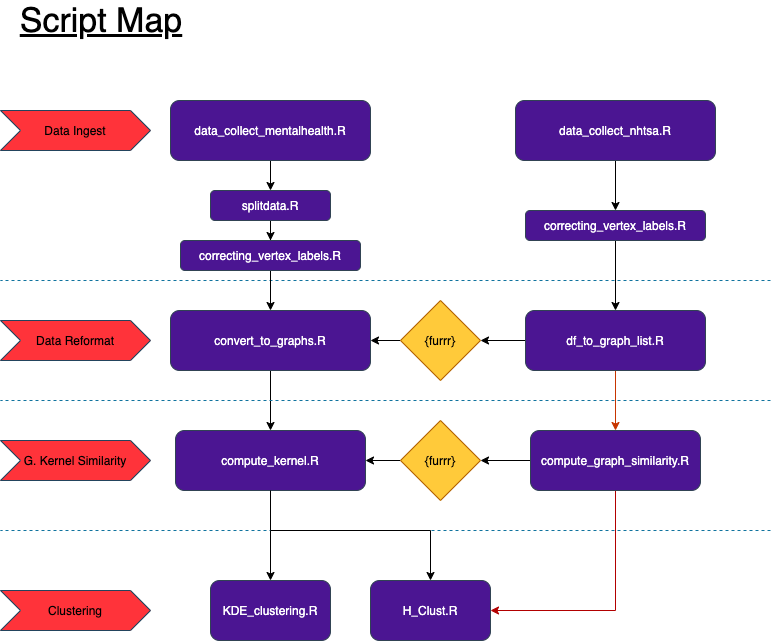
\includegraphics[width=6in]{Content/Images/ScriptMap.png}\\
\caption{Development script map that describes how all modules work together from data ingest to final analysis.}
\end{figure} 

 The Script Map shows how these R scripts can be used for either standard computation, in the case of the NHTSA dataset, or parallel computation, as was used in the reddit dataset. Parallel computation was completed through use of the \texttt{\{furrr\}}, an R package that makes parallization of functions similar to mapping functions from the popular \texttt{\{purrr\}} package. The \texttt{\{furrr\}} package works by splitting the computation among ``workers", or cores, in the CPU. This takes full advantage of the processing capabilities of the machine; instead of letting 1 core do all of the work, we can use many more. Implementation of a parallel option was necessary because computational time for a list of graph objects grows rapidly as the number of graphs in the list increases. A small study was conducted on the reddit dataset to plot this relationship.
 
\begin{figure}
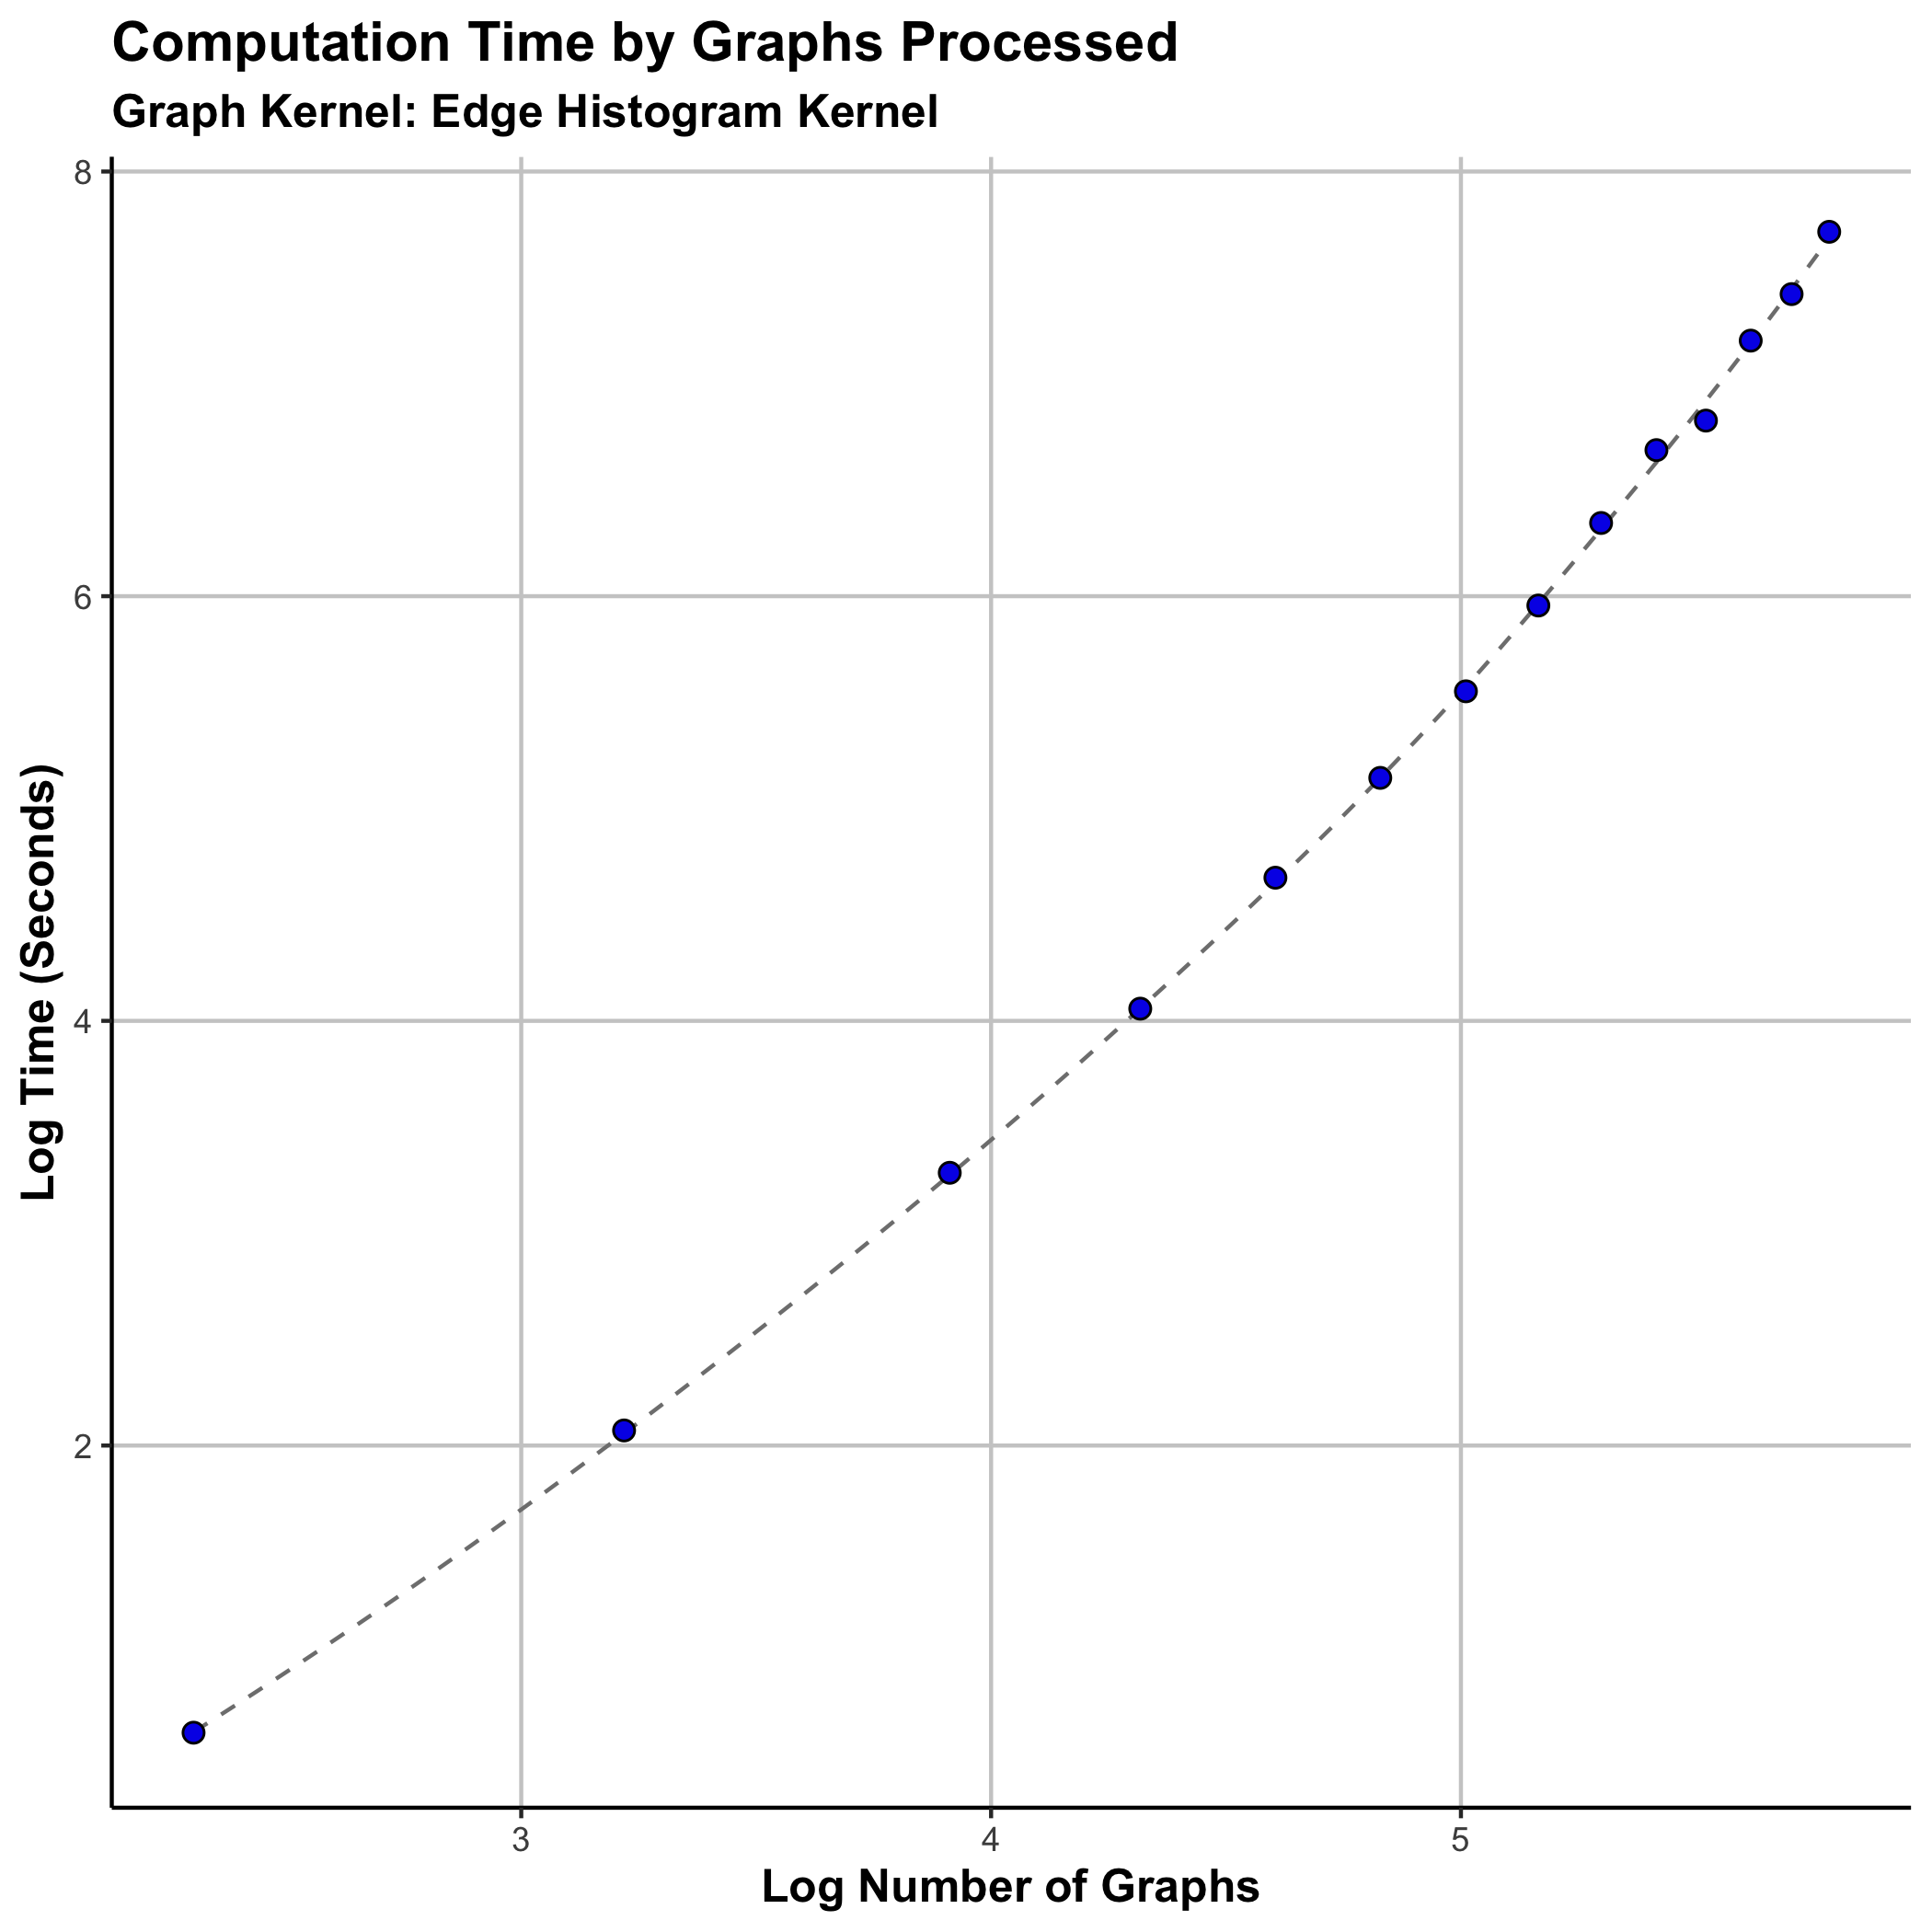
\includegraphics[width=6in]{Content/Images/edgeHistTimePlot.png}\\
\caption{Small study on computation time as a function of the number of graphs in list to be processed. Data from reddit used.}
\end{figure}
 
Above, in Figure 3.2, there is strong evidence that the computation time follows $O(n^2)$. For this reason, the parallel workflow was developed\textemdash to handle datasets with a large number of documents to compare. Even though the amount of text per document in the NHTSA dataset is much larger than the amount of text per document in the reddit dataset, the reddit dataset takes much longer to compute. \\
Referring back to the Script Map, either workflow is decomposed into four steps: Data Ingest, Data Reform, Graph Kernel Similarity, and Clustering. This is the basic work flow developed here. There are some things to note in the Script Map.\\ 
First, vertex labels need corrected to work with the \texttt{\{graphkernels\}} package. This is done through reassignment of all text vertex labels to be a scalar value. The labels are mapped from the union of two graphs' labels to values ranging from $1-n$, where $n$ is the size of the text label set from the union. This script is run within the \texttt{convert\char`_to\char`_graphs.R} script, so it operates on two graphs at a time as it iterates through the whole graph set of concern.\\
Second, the scripts routed through \texttt{\{furrr\}} are functions which are parallelized in the \texttt{convert\char`_to\char`_graphs.R} and \texttt{compute\char`_kernel.R} scripts. These parallelized scripts are done so through a function being executed with no argument, so the dataset which they consider is hard coded into the script. This is not good from a reproducibility aspect, but it is well documented in the code and in the repository, and has reproducible results. \\
Third, the \texttt{splitdata.R} function is there to simply split up the dataset from reddit, which would be too large to store in the repository on GitHub. This segmentation of the data still allows for workflow and reproducibility, since the datasets can all be read in to the environment all the same. \\
Lastly, a KDE clustering analysis was not performed on the NHTSA dataset, as that dataset has few observations ($N=48$) and will not perform well with the density estimation methods developed here; there would be too few observations to generate a number of local maxima/minima needed to apply the clustering methods developed. \\

 

% %---- Chapters
\chapter{Methods}

%\ft{Contents of research work go here.}

%Introduction
%%%%%%%%%%%%%%%%%%%%%%%%
%
%   Thesis template by Youssif Al-Nashif
%
%   May 2020
%
%%%%%%%%%%%%%%%%%%%%%%%%

\section{Introduction}

\ft{Content of the introduction section}

%--- Any subsection will go here.


%%%%%%%%%%%%%%%%%%%%%%%%
%
%   Thesis template by Youssif Al-Nashif
%
%   May 2020
%
%%%%%%%%%%%%%%%%%%%%%%%%

\section{Processing Text into Graphs}

\hspace*{0.3cm} For both datasets, the reddit comments and the SCI papers, the text data is collected and stored in its raw form for reproducibility. The text is then cleaned and prepared for analysis using a suite of text processing tools from the \texttt{\{tidytext\}} package for R \cite{silge2016tidytext}. Using this package, the text undergoes tokenization into skip-grams, stop word removal, and filtering to remove punctuation, numbers, short words, etc. \\

Skip-grams are produced for $k=2,3,4$, where $k$ is the window width of the skip-gram for which bigrams are formed. Stop words are gathered from popular lexicons: ``snowball", ``SMART", and ``onix". As stated above, all numeric values, and lingering punctuation were also removed through use of the \texttt{\{stringR\}} package \cite{wickham2010stringr}. This processing is an essential preprocessing step for using graph kernels to gauge similarity of documents, because words and strings (like punctuation or numbers) that get repeated frequently across many documents in the set do not actually mean the documents are similar\textemdash they just have common reoccurring words. Removing these types of words forces the text data to be more unique across the document set.  \\

The result of the skip-gram tokenizer is a data frame where each observation is a bigram, a pair of words, that the skip-gram window captured. The data frame is then cleaned of stop words through using anti-joins on each bi-gram; any row with the appearance of a stop word in either position, the first or second word, was removed. The same method was applied for punctuation and numbers. The result was a data frame of bigrams which appeared in a fixed window width, $k$, of one another and where both words are of a length greater than 3 letters, not a stop word, and do not contain numbers or punctuation. This cleaned dataset is now ready to be converted into a graph object. \\

Now that the skip-grams are cleaned, the data frame can be converted to a graph object, through use of the \texttt{\{igraph\}} package \cite{csardi2013package}. To do this, each word pair in the data frame is converted to an edge and vertex pair in the graph object. For example, the word pair ``data frame" will become two vertices, labeled ``data" and ``frame", with an undirected edge connecting them. In this study, directed graph edges are not used, but could be considered in future iterations of this work. When this completed for all the skip-gram pairs that were generated, it produces a singular connected graph, however a great deal of filtering occurred and there may be disconnected portions. When words are removed from the graph, a vertex will disappear and can potentially split the graph. This is not too common in the NHTSA dataset for two reasons. First, the text data is quite long, and so if a word is reused at a later time in the text there will be an additional connection to keep it included in the main graph. Secondly, the benefit of the skip-gram, as opposed to plain bigrams, is that the larger window width means words get connected and can ``skip" over words that will get removed through the data cleaning process. So at this point, if there is a group of words that are isolated and not connected to the main graph, they are often quite small and are only several words. To keep computation simple, these lingering small isolated graphs are removed. The vertices that are not members of the main graph are removed from the graph object and that leaves a single connected graph for each text document. These graphs can be compared with graph kernels easily now. 




%%%%%%%%%%%%%%%%%%%%%%%%
%
%   Thesis template by Youssif Al-Nashif
%
%   May 2020
%
%%%%%%%%%%%%%%%%%%%%%%%%

\section{Graph Kernels for Similarity}

Graph kernels can be used to compare the similarity of two graphs. The development of these methods arose out of the need to determine if graphs were isometric in a faster way. The solution was a graph kernel which produces a scalar value for how similar two, or more, graphs are. The result of a graph kernel is a matrix where the similarity of graphs $i$ and $j$ is in the kernel's $i$-th row and $j$-th column entry. This resulting matrix can be used in a variety of ways, but it will be used as a distance matrix in applications here. \\

Amongst graph kernels which consider edge or vertex labels in their computation, various surveys and studies have found edge label histogram kernels or vertex label histograms to be the most efficient. They may not out perform the other methods, like a Weisfeiler-Lehman or other subgraph methods, but they are computationally cheap. The datasets being studied here are both large: one contains many smaller graphs, and one contains 48 very large graphs. So for this study, computation efficiency was prioritized. \\

The edge label histogram kernel is the graph kernel that was chosen for these datasets, and it can be computed using either a linear kernel or a Guassian radial basis function (RBF) kernel between the edge label histograms. \\
An edge label histogram is defined as $\vec{g} = (g_1,g_2, ... g_i)$ such that $g_i = | \{ (u,v) \in E | \phi(u,v) = i \} |$ for each $i$ (CITE SUGIYAMA HALTING KERNELS). Where $g_i$ is a histogram bin for a unique edge label's magnitude, $E$ is the set of edges, and $\phi$ is a function that maps each label to a scalar value in the range of unique values. The edge label histograms are then passed through a kernel, either a linear kernel or a Gaussian RBF kernel.\\
Computation using a linear kernel takes two graphs, $G$ and $G'$, and uses their edge label histograms $\vec{g}$ and $\vec{g'}$. The kernel is computed as:

$$K(\vec{g},\vec{g'}) = \vec{g}^{T}\vec{g'} $$

The resulting value is stored in the graph kernel matrix as the measure of similarity between the two graphs in the corresponding row and column for the pair. (CITE SUGIYAMA)

Alternatively, the Gaussian RBF kernel takes the edge label histograms of $G$ and $G'$, that we call $\vec{g}$ and $\vec{g'}$, and the kernel is computed as:

$$K(\vec{g},\vec{g'}) = e^{-(\frac{||\vec{g}- \vec{g'}||^2}{2 \sigma^2})}$$

The resulting value is stored in the graph kernel matrix as the measure of similarity between the two graphs in the corresponding row and column for the pair. (CITE SUGIYAMA)\\

Through either of these kernels, we obtain a kernel of dimensions $n \times n$ for a list of $n$ graphs. This kernel can then be used for clustering methods.

% https://papers.nips.cc/paper/2015/file/31b3b31a1c2f8a370206f111127c0dbd-Paper.pdf




%%%%%%%%%%%%%%%%%%%%%%%%
%
%   Thesis template by Youssif Al-Nashif
%
%   May 2020
%
%%%%%%%%%%%%%%%%%%%%%%%%

\section{Graph Kernels for Similarity}

The resulting graph kernel matrix, with dimensions $n \times n$, is high dimensional data. We can take this kernel and perform a principal component analysis (PCA) to reduce the high dimensionality of this data. Each row, can be considered as an observation, and each column as it's similarity value or in the $j$-th graph's dimension. PCA then allows us to express the data in a lower dimensionality, hopefully in 2 or 3 dimensions which can be visualized much better. \\
Then, 


%%%%%%%%%%%%%%%%%%%%%%%%
%
%   Thesis template by Youssif Al-Nashif
%
%   May 2020
%
%%%%%%%%%%%%%%%%%%%%%%%%

\section{Alternate Clustering Method with KDE}

As an alternative to popular clustering methods that were used in the preceding section, another clustering method was attempted that features use of kernel density estimation. By using a kernel density estimation (KDE) on the kernel values, we can cluster the documents into similar groups, defined by local maxima. \\
First, the graph kernel matrix, $K$ is taken, and we extract a row, $i$, and we compute a KDE using R's \texttt{density()} function. Now, the default value for bandwidth will likely produce a smooth, unimodal or bimodal distribution, but this is not what the goal is. The goal is to use the KDE to find clusters through their value appearing in a local maxima. So, through producing a KDE with few local maxima, we produce very few clusters. If the number of clusters needs to increase, we can essentially overfit the KDE and abuse the use of the bandwidth parameter to create a KDE with many more local maxima and minima.\\

%% INSERT GRAPHIC HERE.
**GRAPHIC**\\ 

Once a KDE with a sufficient number of local maxima, which is determined by the user, then cluster breaks are located. If we consider the estimated KDE to be a function $k(x)$, where $x$ is a kernel value, and $k(x)$ is the estimated density at a value $x$, then we can do calculus to locate the break points. 



\section{Development of Methods}

All of the methods outlined in preceding chapters were developed in \textit{RStudio} and are stored in a public code repository on \textit{GitHub}. Initial development and testing of all the packages and libraries was completed using \textit{R Markdown} notebooks, which allow for coding in chunks with explanation in markdown text. These netbooks are kept in the code repo to serve as more explanatory documents demonstrating how all the scripts and datasets work in conjunction with one another. \\
The resulting and final scripts are kept in the code repository as well. The final scripts were developed to use the output from one another and to produce intermediate outputs so that small studies could be conducted. How the scripts work with one another is mapped out in the "Script Map" in Figure 3.1.\\

\begin{figure}
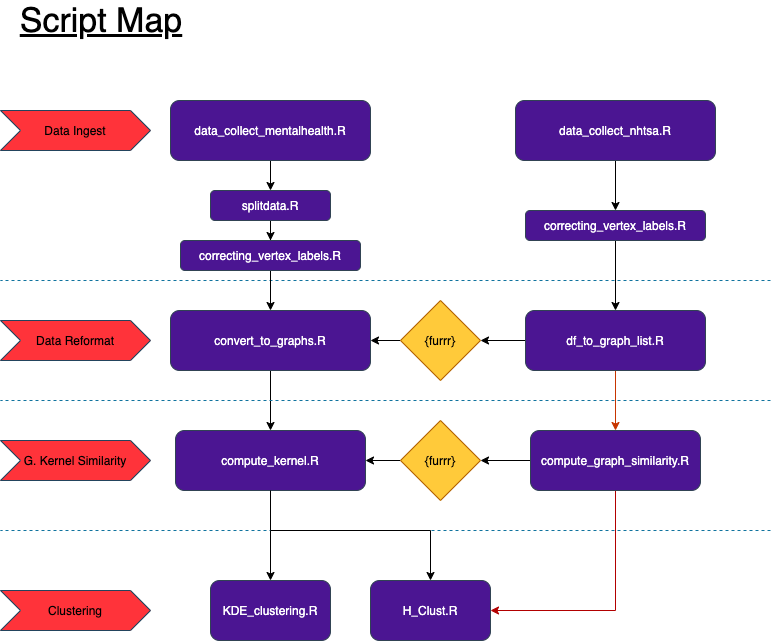
\includegraphics[width=6in]{Content/Images/ScriptMap.png}\\
\caption{Development script map that describes how all modules work together from data ingest to final analysis.}
\end{figure} 

 The Script Map shows how these R scripts can be used for either standard computation, in the case of the NHTSA dataset, or parallel computation, as was used in the reddit dataset. Parallel computation was completed through use of the \texttt{\{furrr\}}, an R package that makes parallization of functions similar to mapping functions from the popular \texttt{\{purrr\}} package. The \texttt{\{furrr\}} package works by splitting the computation among ``workers", or cores, in the CPU. This takes full advantage of the processing capabilities of the machine; instead of letting 1 core do all of the work, we can use many more. Implementation of a parallel option was necessary because computational time for a list of graph objects grows rapidly as the number of graphs in the list increases. A small study was conducted on the reddit dataset to plot this relationship.
 
\begin{figure}
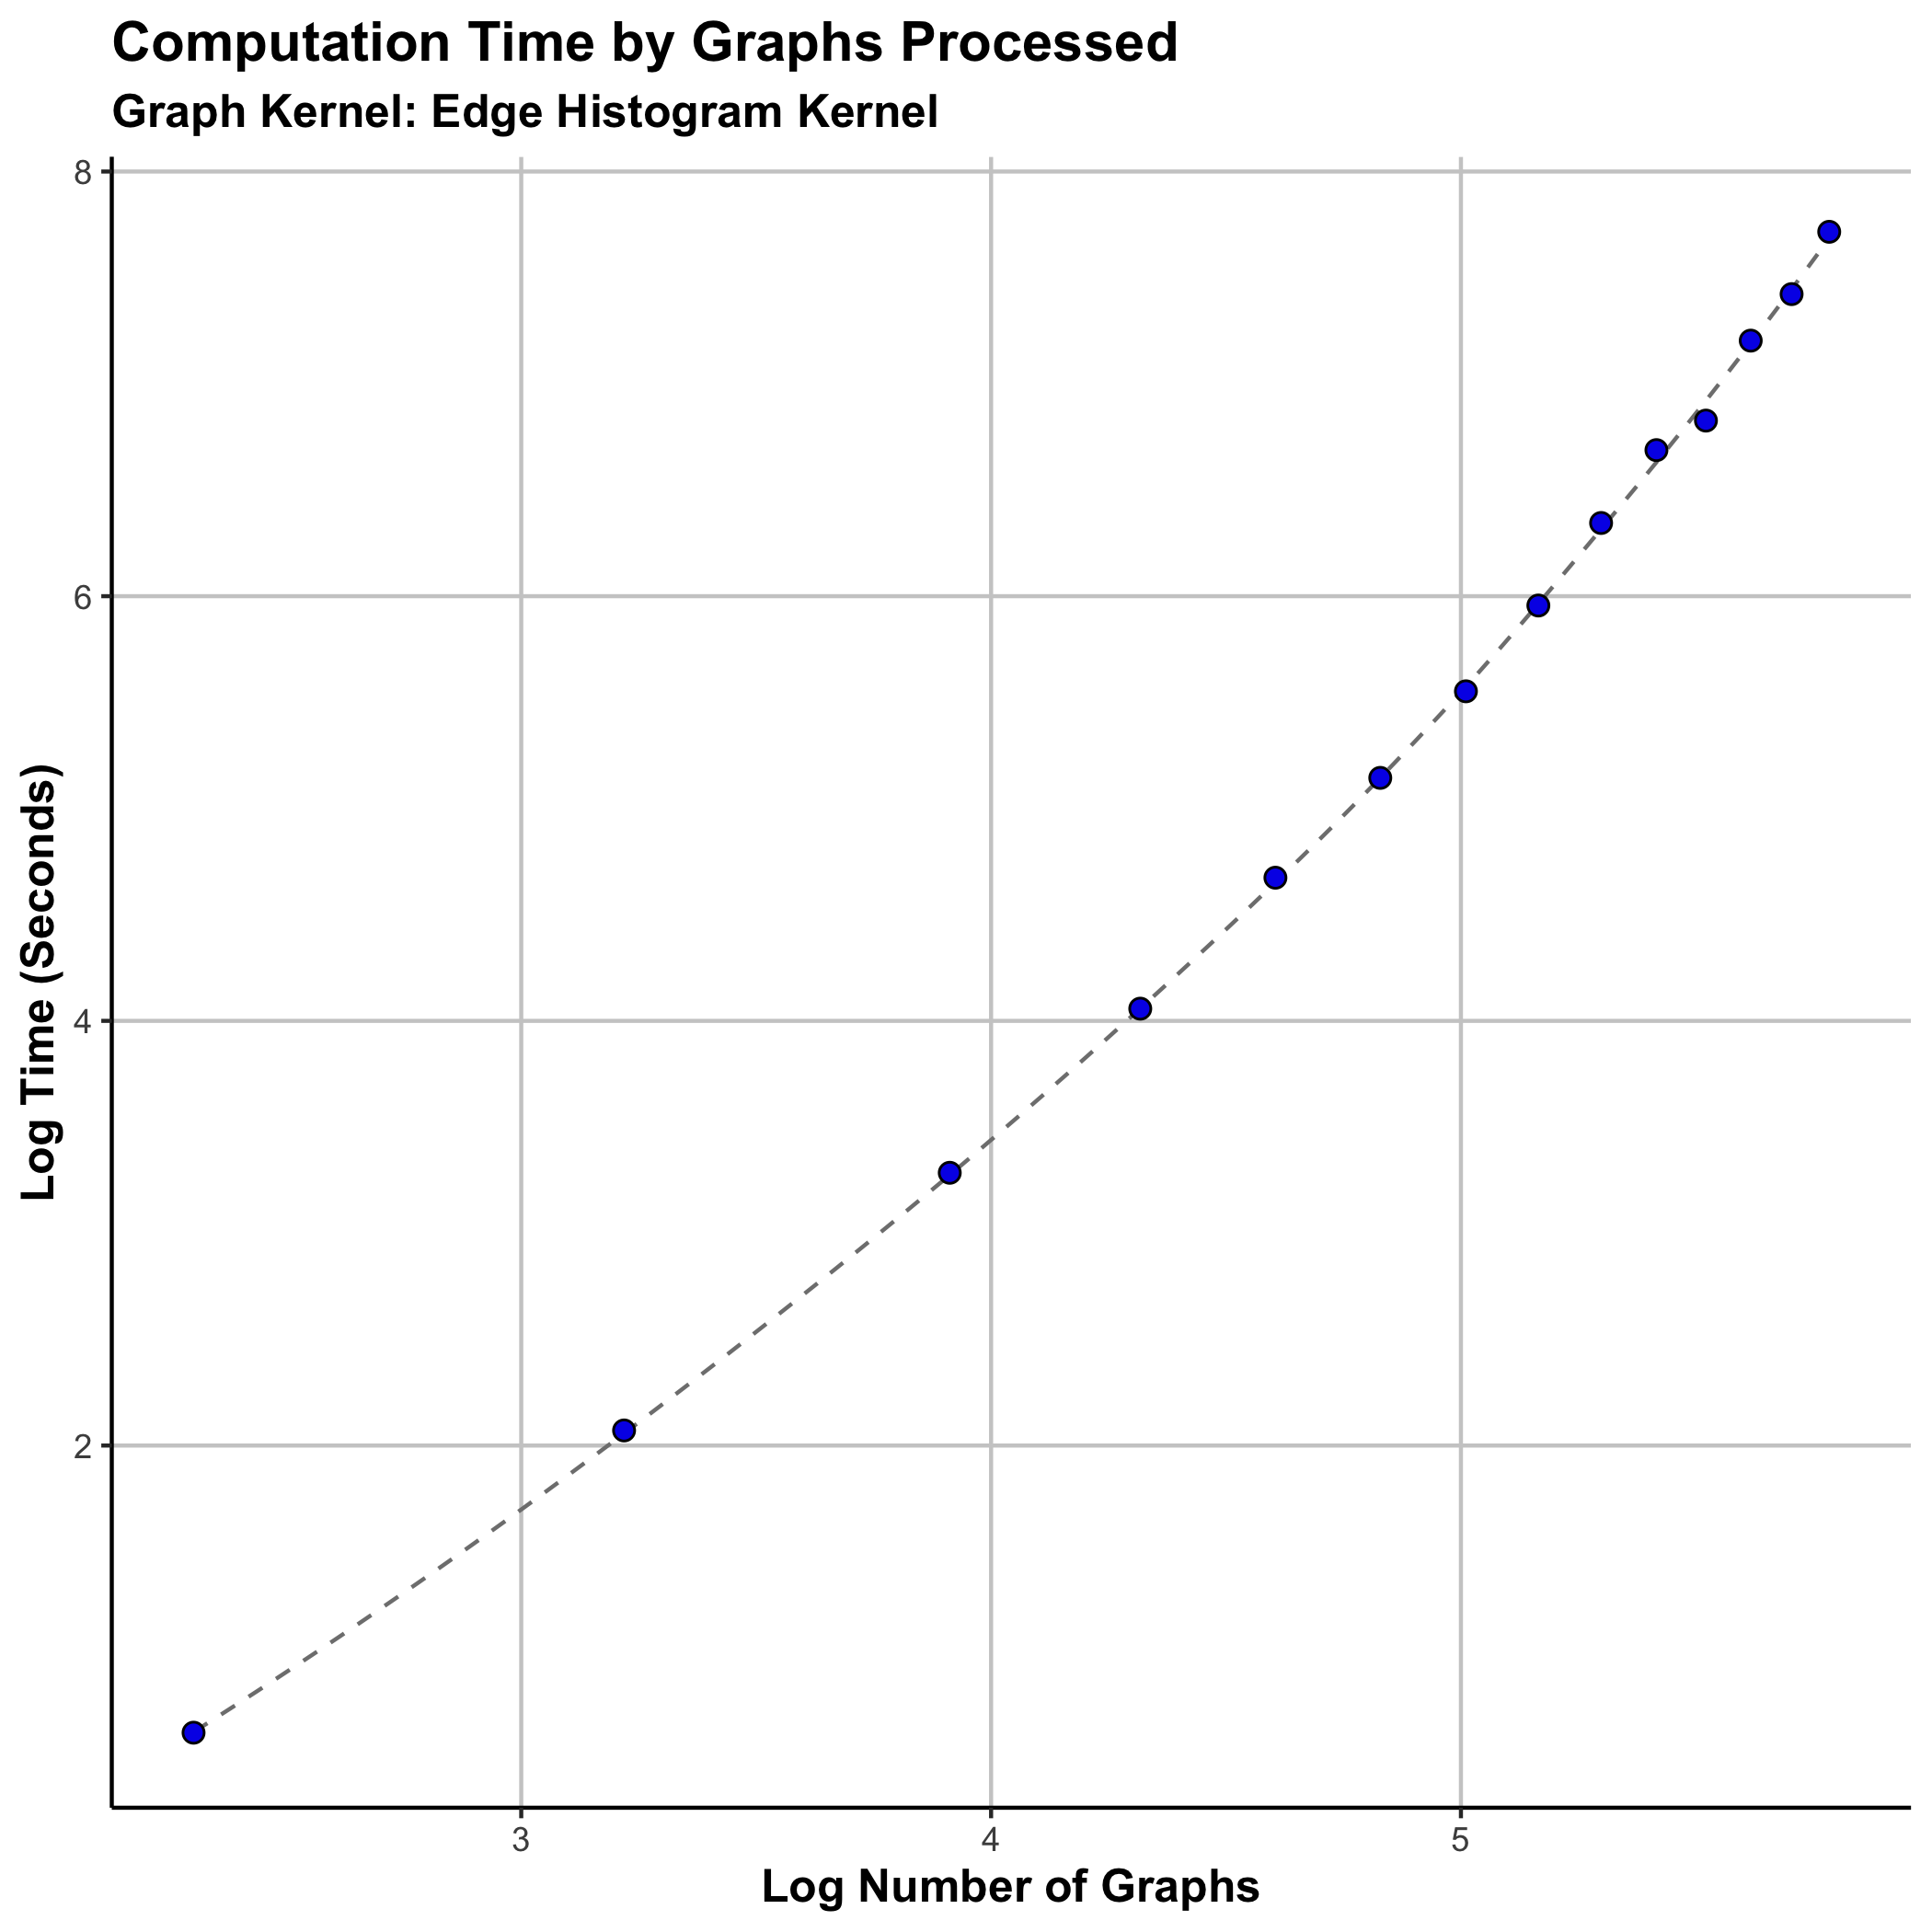
\includegraphics[width=6in]{Content/Images/edgeHistTimePlot.png}\\
\caption{Small study on computation time as a function of the number of graphs in list to be processed. Data from reddit used.}
\end{figure}
 
Above, in Figure 3.2, there is strong evidence that the computation time follows $O(n^2)$. For this reason, the parallel workflow was developed\textemdash to handle datasets with a large number of documents to compare. Even though the amount of text per document in the NHTSA dataset is much larger than the amount of text per document in the reddit dataset, the reddit dataset takes much longer to compute. \\
Referring back to the Script Map, either workflow is decomposed into four steps: Data Ingest, Data Reform, Graph Kernel Similarity, and Clustering. This is the basic work flow developed here. There are some things to note in the Script Map.\\ 
First, vertex labels need corrected to work with the \texttt{\{graphkernels\}} package. This is done through reassignment of all text vertex labels to be a scalar value. The labels are mapped from the union of two graphs' labels to values ranging from $1-n$, where $n$ is the size of the text label set from the union. This script is run within the \texttt{convert\char`_to\char`_graphs.R} script, so it operates on two graphs at a time as it iterates through the whole graph set of concern.\\
Second, the scripts routed through \texttt{\{furrr\}} are functions which are parallelized in the \texttt{convert\char`_to\char`_graphs.R} and \texttt{compute\char`_kernel.R} scripts. These parallelized scripts are done so through a function being executed with no argument, so the dataset which they consider is hard coded into the script. This is not good from a reproducibility aspect, but it is well documented in the code and in the repository, and has reproducible results. \\
Third, the \texttt{splitdata.R} function is there to simply split up the dataset from reddit, which would be too large to store in the repository on GitHub. This segmentation of the data still allows for workflow and reproducibility, since the datasets can all be read in to the environment all the same. \\
Lastly, a KDE clustering analysis was not performed on the NHTSA dataset, as that dataset has few observations ($N=48$) and will not perform well with the density estimation methods developed here; there would be too few observations to generate a number of local maxima/minima needed to apply the clustering methods developed. \\

 



\bibliographystyle{apacite}
\bibliography{Bibliography/bibliography.bib}



\end{document}
